\section{Approach}
\label{sec:approach}

In this section, we present our approach for detecting malicious behaviors embedded in model artifacts. The pipeline operates in three stages: (i) \emph{Data Collection}, which gathers two synchronized evidence streams—low-level system-call traces and high-level Python semantic logs; (ii) \emph{Coarse-grained Filtering}, which clusters raw system calls into operation vectors, screens for anomalies via an unsupervised autoencoder, and retrieves aligned semantic context through fuzzy spatio-temporal matching; and (iii) \emph{Fine-grained Verification}, where an LLM jointly reasons about the system-call evidence and Python semantic context to produce an intent score, a threat category, and an auditable evidence chain.

\begin{figure*}[t!]
    \centering
    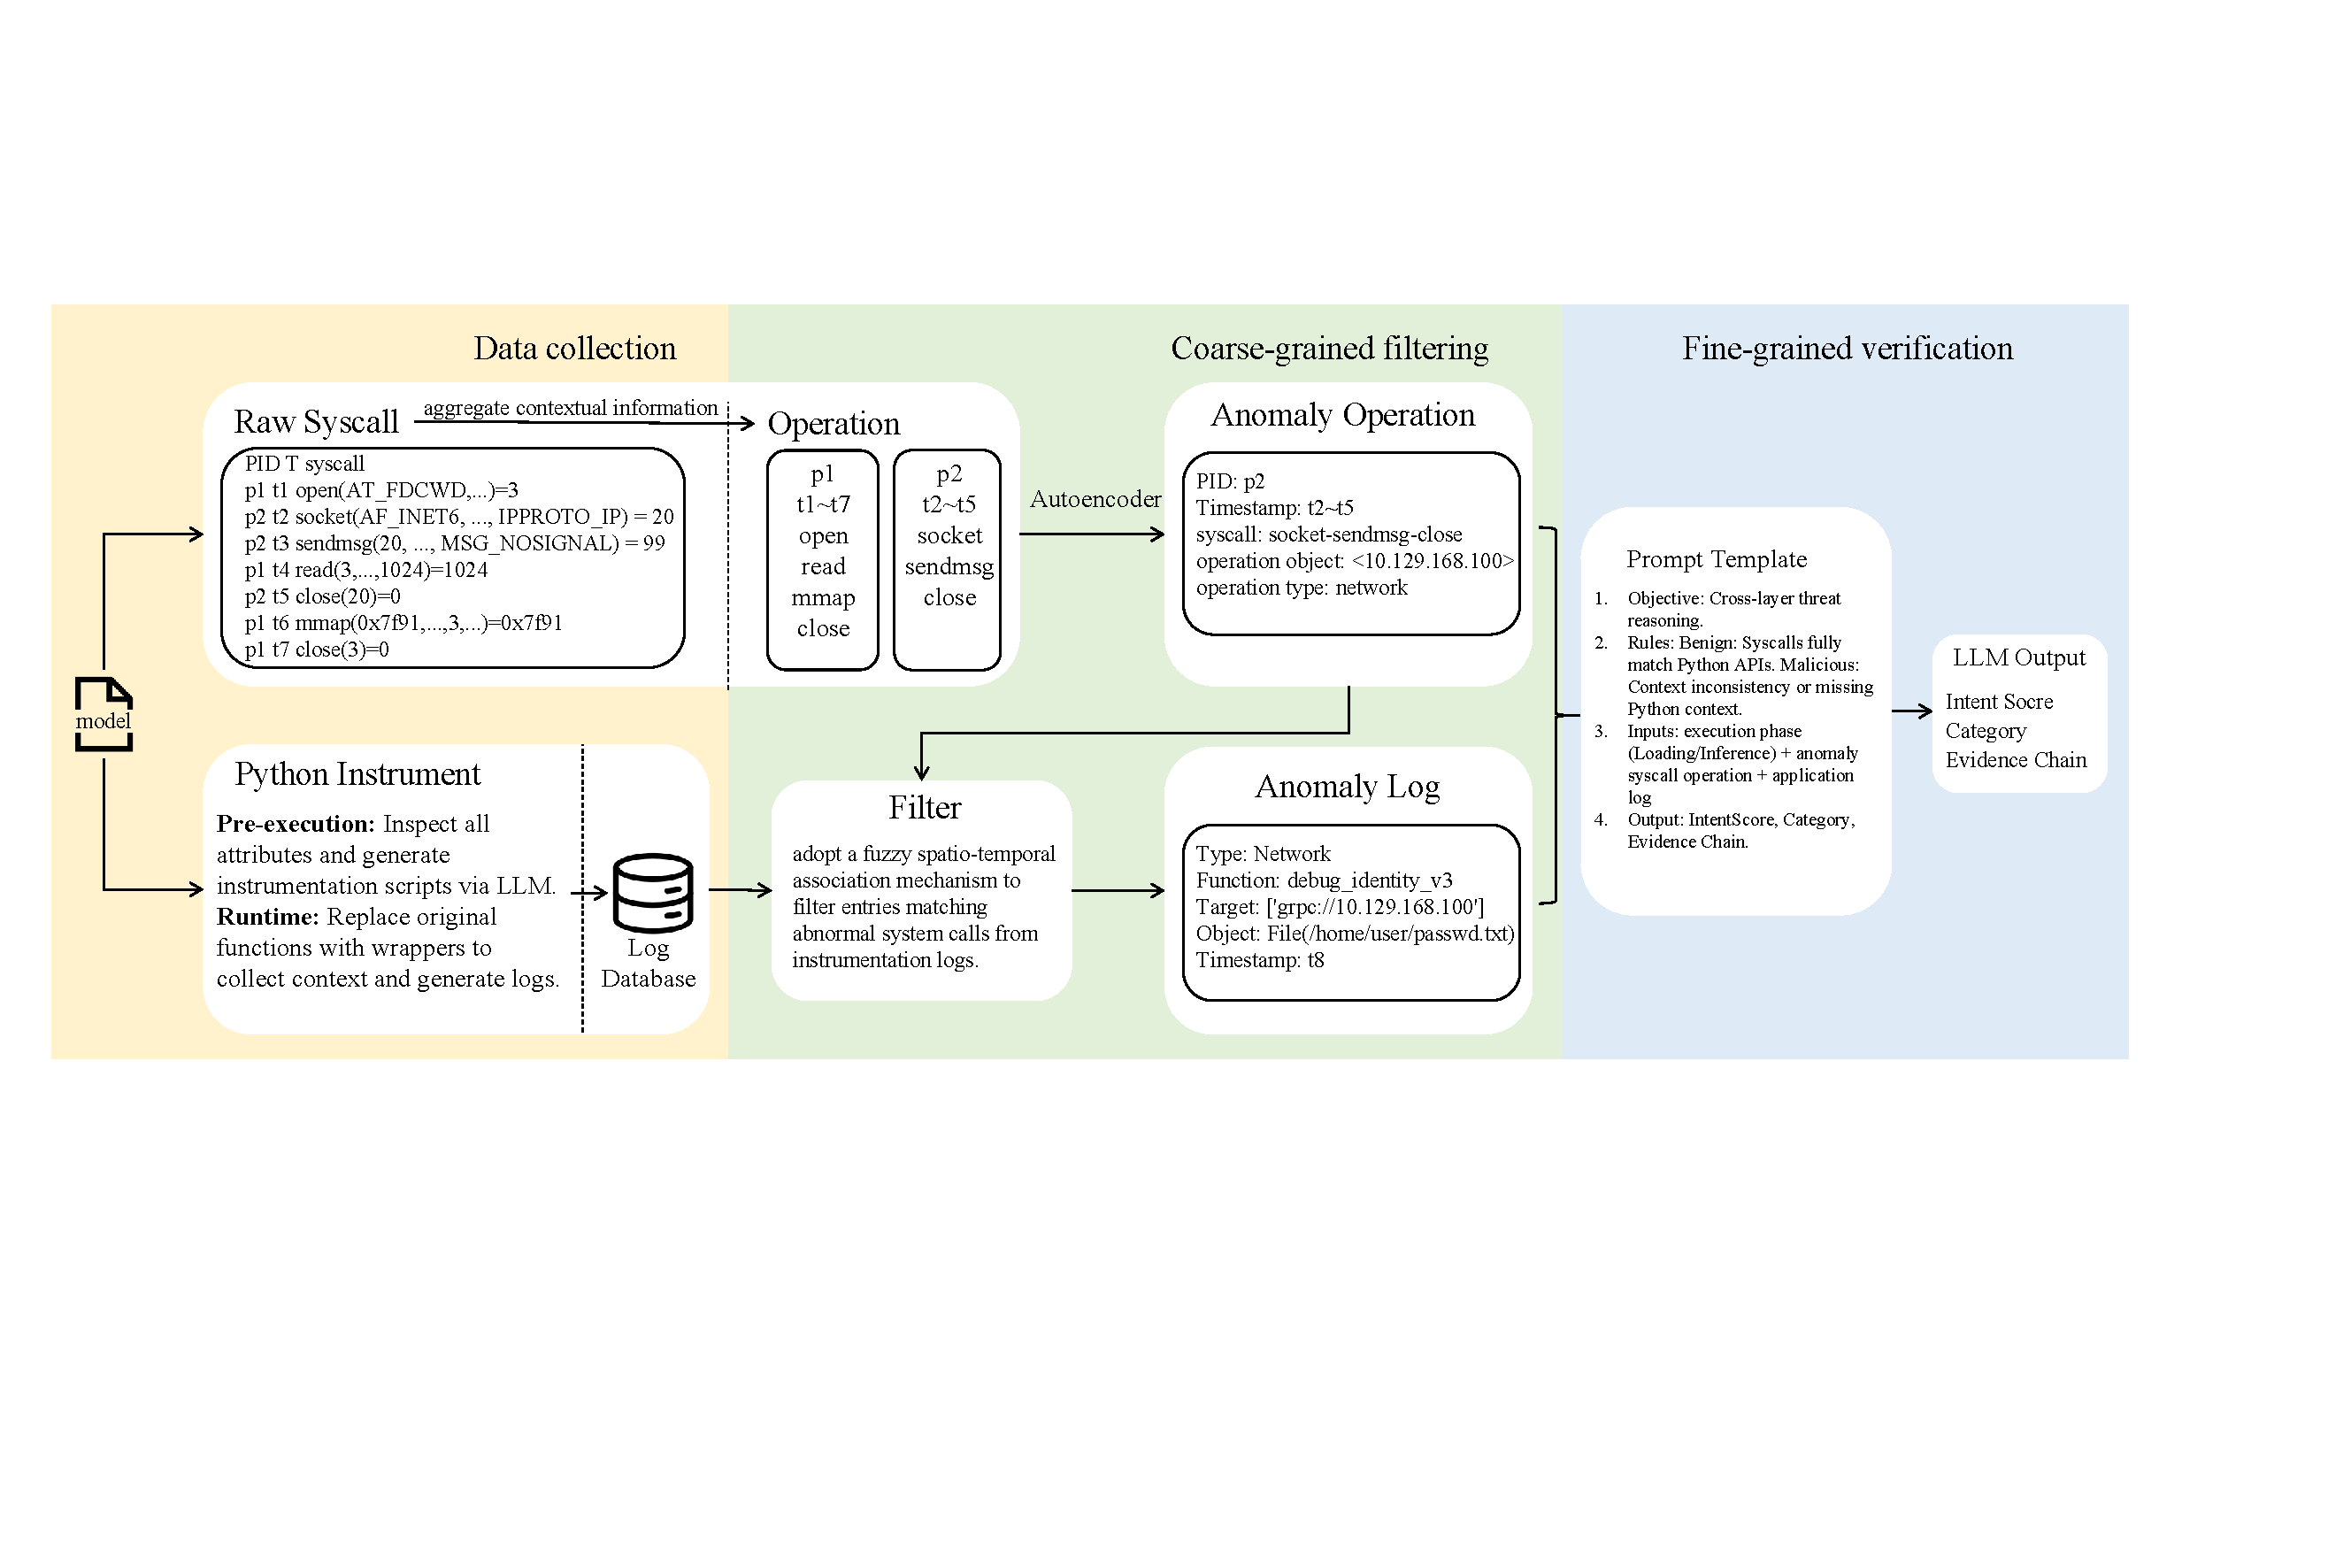
\includegraphics[width=\linewidth]{figs/overview3.pdf}
    \caption{Overview of the hybrid defense system.}
    \label{fig:overview}
\end{figure*}

\subsection{Data Collection}

The data collection stage simultaneously captures two synchronized streams of evidence during controlled model execution: a kernel-visible system-call stream and an application-layer semantic log stream. Together, these streams provide the complementary low-level and high-level signals needed for downstream analysis.

\subsubsection{System-call collection.}
We base our detection on system-call traces because they operate below the user-space level and cannot be bypassed by any Python-level obfuscation~\cite{2875487}: no matter how a model artifact hides its malicious intent through code mangling or dynamic loading, its actual interactions with the operating system must traverse the kernel and therefore leave a non-bypassable forensic record.

\begin{table}[t!]
	\centering
	\caption{Security-relevant system-call categories used by our filter.}
	\begin{tabular}{l p{0.28\columnwidth} p{0.45\columnwidth}}
		\hline
		Filter param & Category & Purpose \\
		\hline
		file   & File operations (\texttt{read}/\texttt{write}) & Detect sensitive data leakage or configuration file tampering \\
		network & Network operations (\texttt{socket}) & Detect data exfiltration or remote command execution \\
		cred   & Credential operations (\texttt{setuid}) & Detect privilege-escalation behavior \\
		desc   & Descriptor operations (\texttt{dup}) & Assist file-related anomaly detection \\
		signal & Signal handling (\texttt{kill}) & Capture malicious process termination attempts \\
		clock  & Time-related operations & Assist temporal anomaly analysis (e.g., abnormal delays) \\
		\hline
	\end{tabular}
	\label{tab:syscalltypes}
\end{table}

We employ a selective tracing strategy that focuses exclusively on security-relevant system-call families, discarding high-frequency but semantically uninformative calls to keep the trace volume manageable. During controlled model execution, we use \texttt{strace} to continuously trace system calls of the target process. To reduce noise and overhead, we immediately discard calls such as scheduler hints and memory-mapping operations that carry no security signal\cite{shakya2022analysisdetectionclassificationandroid}. The selection concentrates on system-call categories that can indicate malicious intent. Table~\ref{tab:syscalltypes} summarizes the security-relevant syscall families we monitor and their roles in our detection pipeline. For example, file operations can reveal attempts to access sensitive data or modify configurations, while network operations may signal data exfiltration or remote command execution.

\subsubsection{Instrumentation log collection.}
To bridge the semantic gap between model-level intent and kernel-level behavior, we collect high-dimensional Python semantic context via non-invasive instrumentation. The key challenge is that heterogeneous ML frameworks expose frequently changing APIs, making manual per-framework instrumentation labor-intensive and coverage-incomplete. We address this through an LLM-assisted approach with two distinct phases.

\noindent \textbf{Pre-execution: API Discovery and Script Generation.}
Before model execution, we leverage an LLM to synthesize dynamic instrumentation scripts. A rigorously structured prompt constrains the LLM to generate code that inspects the target module's namespace at startup, systematically identifies all public callable attributes, and constructs wrapper closures around each. The prompt specifies the security objective, mandates capturing execution context which contains timestamps, operation types, argument values and return types, and requires all intercepted events to be serialized into standardized JSON. This automated discovery eliminates statically hardcoded API lists and adapts to framework version changes by simply regenerating wrappers for the new API surface, without modifying the core detection pipeline.

Algorithm~\ref{alg:instrumentation} formalizes this discovery and wrapping logic. The \texttt{ApplyDynamicPatches} procedure isolates public callables while skipping private attributes and non-callable objects, then generates wrapper closures for each target API.

\begin{algorithm}[t!]
\caption{Automated Dynamic Instrumentation Logic}
\label{alg:instrumentation}
\KwIn{Target library module $\mathcal{M}$ (e.g., \texttt{torch}, \texttt{tensorflow})}
\KwOut{Instrumented module capable of context logging}

\SetKwProg{Fn}{Procedure}{:}{}
\SetKwFunction{FApply}{ApplyDynamicPatches}
\SetKwFunction{FConstruct}{Wrapper}

\Fn{\FApply{$\mathcal{M}$}}{
    \ForEach{attribute name $attr\_name$ \textnormal{\textbf{in}} \textnormal{dir}($\mathcal{M}$)}{
        \If{$attr\_name$ starts with ``\_''}{
            \textbf{continue} 
        }
        
        $target\_func \gets$ \textnormal{getattr}($\mathcal{M}, attr\_name$)\;
        \If{\textnormal{\textbf{not}} is\_callable($target\_func$)}{
            \textbf{continue} 
        }
        
        $wrapper \gets$ \FConstruct{$target\_func, attr\_name$}\;
        
        \textbf{try}\;
        \Indp \textnormal{setattr}($\mathcal{M}, attr\_name, wrapper$)\; 
        \Indm \textbf{catch} \textit{ReadOnlyAttributeError} \;
        \Indp \textbf{continue} \;
        \Indm
    }
}
\Fn{\FConstruct{$func, name$}}{
    \KwRet a closure that captures the full \texttt{traceback}, logs to JSON, executes $func$, and delegates return value\;
}
\end{algorithm}

\noindent \textbf{Runtime: Wrapper Injection and Context Logging.}
At process startup, the generated script employs monkey patching (\texttt{setattr}) to replace original functions with wrapper closures. Thereafter, any invocation of a wrapped API triggers the injected closure, which captures the execution context and serializes it as a structured semantic event:
\begin{equation}
\ell_i = \langle \textit{FuncName},\; \textit{ArgsSummary} \rangle.
\end{equation}
Here $\textit{FuncName}$ denotes the invoked framework or standard-library API, while $\textit{ArgsSummary}$ aggregates only lightweight information—tensor shapes and dtypes, configuration flags, truncated or hashed file paths, and bounded-length string summaries—controlling logging overhead while preserving rich contextual signals.

To ensure runtime safety, wrappers follow a conservative policy: they only wrap callable functions avoiding class definitions, built-in types, and C/C++ bindings, perform best-effort argument summarization without altering return values or side effects, and employ defensive serialization. The patching process is additionally wrapped in \texttt{try-except} blocks to survive read-only properties, immutable C-extension bindings, and dynamically generated descriptors that would otherwise crash the process. Any patch failure degrades gracefully without disrupting the target process.

\subsection{Coarse-grained Filtering}

After collecting raw evidence streams, the coarse-grained filtering stage transforms system-call traces into compact operation vectors, screens for anomalies, and retrieves the corresponding semantic context. This stage eliminates clearly benign activity before the expensive LLM reasoning stage.

\subsubsection{System-call Clustering and Embedding}

The collected system-call traces are extremely fine-grained and voluminous. A single model loading process may produce thousands of system calls, and meaningful malicious behavior invariably manifests as a \emph{sequence} of related calls rather than as isolated events. To address this, we aggregate correlated system calls into compact, high-level operation vectors that reduce trace noise, compress data volume, and provide standardized analysis units with complete semantics for downstream anomaly detection.

To accurately model the execution semantics of a program, it is crucial to recognize that system calls inherently possess varying degrees of contextual dependency. Applying a uniform extraction strategy to all system calls would be ineffective: some operations are semantically self-contained and immediately indicative of high-risk behavior, whereas others are granular, stateful operations that remain ambiguous unless analyzed as a continuous sequence. Motivated by this fundamental difference, we propose a hybrid embedding scheme that categorizes the traced system calls into two distinct streams for targeted handling: (1) \emph{Directly malicious calls} and (2) \emph{Stateful calls}. By processing these two streams individually, we ultimately synthesize them into a unified feature space for downstream analysis.

\noindent \textbf{Direct call embedding.}
The first category includes standalone, high-risk operations (e.g., \texttt{execve}, \texttt{chmod}) that do not require lifecycle context. We directly encode each of these calls into a fixed-dimension operation vector $\mathbf{v}_{\textit{dir}} \in \mathbb{R}^{d}$. Specifically, we utilize a pre-trained BERT-based model to extract the rich semantic meaning from the call's underlying logic and literal arguments. This high-dimensional representation is subsequently projected down to the target dimension $d$, ensuring that semantically critical, self-contained threats are instantly captured without the need for sequence aggregation.

\noindent \textbf{Stateful aggregation.}
Let $S = \{(s_k, \tau_k)\}_{k=1}^{N}$ denote the traced system-call stream, where $s_k$ is the $k$-th syscall and $\tau_k$ its timestamp. For stateful operations, we maintain per-resource state keyed by $r = \langle \textit{PID}, \textit{FD} \rangle$, where $\textit{FD}$ denotes a file or socket descriptor. For each key $r$, we collect the indices of calls that operate on this resource within one lifecycle segment,
\begin{equation}
I_r = \{\, k \mid (s_k, \tau_k) \in S,\ s_k \text{ uses resource } r,\ \tau_{\textit{start}}^r \le \tau_k \le \tau_{\textit{end}}^r \,\},
\end{equation}
where $\tau_{\textit{start}}^r$ and $\tau_{\textit{end}}^r$ are the timestamps of the resource-acquisition and resource-release calls (e.g., \texttt{open} / \texttt{close} or \texttt{socket} / \texttt{shutdown}). The lifecycle segment for resource $r$ is then the ordered subsequence $S_r = \{(s_k, \tau_k)\}_{k \in I_r}$.

We aggregate this segment into a fixed-length operation vector by applying a feature-extraction function $\phi$ over all calls in the segment:
\begin{equation}
\mathbf{v}_{\textit{sys}}(r) = \phi(S_r) \in \mathbb{R}^{d},
\end{equation}
where $\phi$ operates by extracting the common resource identifier $r = \langle \textit{PID}, \textit{FD} \rangle$ shared across the segment $S_r$, and concatenating it with the sequence of distinct, call-specific parameters (e.g., flags, buffer sizes, or return values) derived from each individual system call $s_k \in S_r$. This concatenated feature sequence is subsequently passed through an embedding layer to project it into the continuous $\mathbb{R}^{d}$ space. Intuitively, each $\mathbf{v}_{\textit{sys}}(r)$ captures a dense, contextualized representation of the exact data flow and state transitions associated with a specific file or connection during its lifetime, effectively smoothing out scheduling artifacts and interleaving from other threads.

The final feature matrix combines $\mathbf{v}_{\textit{dir}}$ and $\mathbf{v}_{\textit{sys}}$, enabling the system to capture both direct and aggregated syscall behaviors. This hybrid representation ensures that directly malicious actions are immediately flagged, while stateful operations are analyzed in context to detect more subtle threats.

\subsubsection{Autoencoder-based Anomaly Detection}

We adopt unsupervised anomaly detection because benign model loading and inference produce a stable, learnable distribution of system-call operations, whereas malicious behaviors are inherently rare and diverse, making supervised classification impractical without labeled attack samples that cover the full threat space. Among unsupervised methods, we choose an Autoencoder for its conceptual simplicity and proven effectiveness in reconstruction-based anomaly detection: it learns to faithfully reconstruct benign operation vectors during training and naturally flags any vector it cannot faithfully reconstruct as anomalous.

We train an Autoencoder on operation vectors collected from clean model loading and inference runs. Given an operation vector $\mathbf{v}$, the Autoencoder computes a reconstruction error
\begin{equation}
E = \left\lVert \mathbf{v} - \textit{Dec}(\textit{Enc}(\mathbf{v})) \right\rVert_2^2,
\end{equation}
where \textit{Enc} and \textit{Dec} denote the encoder and decoder networks, respectively. Operations with reconstruction error $E$ below a threshold $\theta$ are treated as consistent with normal model behavior and are discarded. If $E > \theta$, we mark the corresponding operation as abnormal, retain its full underlying system-call segment $S'$ and metadata $\langle \textit{PID}, \textit{TID}, t_{\textit{start}}, t_{\textit{end}} \rangle$, and promote it to the subsequent spatio-temporal matching stage.

By performing this unsupervised prefiltering at the operation level, the system keeps the expensive cross-layer association and LLM reasoning off the critical path for the vast majority of benign activity, while still surfacing rare, suspicious low-level behaviors that deviate from the learned distribution of normal AI model execution.

\subsubsection{Spatio-temporal Semantic Matching}

After the autoencoder identifies abnormal operations, we must determine whether each anomaly can be explained by benign Python-level behavior. This requires retrieving the semantic context from the instrumentation log stream that corresponds to each abnormal system-call operation.

System calls and Python semantics are inherently asynchronous due to operating system scheduling and concurrent I/O. As a result, naive one-to-one timestamp matching between system-call logs and semantic logs is unreliable in high-concurrency workloads. We therefore adopt a fuzzy spatio-temporal association strategy.

For each abnormal operation, the autoencoder screening stage provides the underlying system-call segment $S'$ and its metadata $\langle \textit{PID}, t_{\textit{start}}, t_{\textit{end}} \rangle$. Given this metadata and the semantic log stream $L = \{(\ell_i, t_i)\}$, we perform filtering following the spatial-temporal matching rules below.

\noindent \textbf{Temporal windowing.}
We apply a slack temporal window around the abnormal operation. For each candidate abnormal operation, we define its active time span $[t_{\textit{start}}, t_{\textit{end}}]$ based on the first and last system call in $S'$, and search semantic events whose timestamps $t_i$ fall into an expanded window $[t_{\textit{start}} - \Delta t, t_{\textit{end}} + \Delta t]$. The slack parameter $\Delta t$ tolerates minor scheduling jitter while still localizing semantic context to the period when the resource was actually in use.

\noindent \textbf{Spatial hints.}
Temporal proximity alone is insufficient under heavy concurrency. We therefore further filter candidates using resource-related hints derived from both layers, such as whether the operation is file- or network-related, file paths or prefixes, remote destinations, and other descriptor metadata when available. Combining temporal and spatial constraints yields a fuzzy but robust alignment that significantly reduces spurious associations when many model components execute in parallel.

\subsection{Fine-grained Verification}

Operations that survive coarse-grained filtering are escalated to the fine-grained verification stage, which jointly reasons about the low-level system-call evidence and high-level semantic context to produce a final intent judgment.

Determining whether abnormal low-level operations reflect benign model behavior or malicious intent is inherently challenging: the same system-call pattern can arise from legitimate model loading or from an attacker's attempt to exfiltrate data, and without semantic context the two are indistinguishable at the kernel level. To resolve this ambiguity, we feed each abnormal operation together with its aligned semantic contexts into an LLM, which judges whether the behavior is consistent with benign model execution.

\noindent \textbf{Prompt construction.}
We translate the aligned evidence into a structured natural-language prompt that includes: (i) a concise summary of the abnormal operation including operation type, key statistics, and risk-relevant parameters, (ii) the aligned semantic call contexts including library/API, call stack summary, and argument summaries, and (iii) the execution phase categorized into the model loading stage and inference stage.

Our maliciousness judgment follows a principled cross-layer reasoning rule: a behavior is classified as benign only when its low-level system-call activity can be plausibly explained by the aligned Python-level semantic context. Concretely, if the LLM identifies that the observed file reads, network connections, or process creations are consistent with the framework APIs and execution phase reported in the semantic log, the operation is deemed benign and discarded. Conversely, when inconsistencies exist between the Python-layer semantic logs and the corresponding system-call activities, such as a network connection to an external host with no matching high-level API invocation, or when no matching Python semantic context can be retrieved at all, the behavior is marked as malicious and escalated.

\noindent \textbf{Decision and explanation.}
The LLM outputs $\textit{IntentScore}$, a $\textit{ThreatCategory}$ label, and a rationale. Importantly, we persist the subset of semantic events and system-call summaries used in the reasoning as the \emph{evidence chain} $\textit{Context}$ for auditing.
If high-risk system-call patterns appear without any plausible semantic explanation, the system raises a high-severity alert and can block execution in the controlled environment.


\subsection{Model Vetting Pipeline}
%% [Deployment: \toolname{} operates in pre-deployment fuzzing pipeline, not production serving]

\toolname{} is designed to operate in a pre-deployment model vetting pipeline rather than in production inference serving. Before a model is released or integrated into any production system, it should undergo a comprehensive security vetting phase in a controlled sandbox environment with \toolname{} monitoring its behavior to detect embedded malicious logic.

To maximize detection coverage, we recommend exhaustive fuzzing-based testing of all real-world business workflows that the model will encounter post-deployment\cite{wu2026chainfuzzergreyboxfuzzingworkflowlevel, BAMOHABBATCHAFJIRI2024103903}. Concretely, the model should be exercised through every anticipated usage scenario: loading with all expected input shapes and data types, invoking inference across the full range of supported batch sizes, exercising all serialization, checkpointing, and fine-tuning paths, and simulating edge-case inputs that stress runtime boundaries. This fuzzing strategy ensures that dormant malicious payloads—which may be conditionally triggered only under specific runtime conditions, input patterns, or execution phases—are activated and exposed during testing, providing comprehensive coverage beyond simple model loading.
